\documentclass[times, utf8, seminar, numeric]{fer}

\usepackage{booktabs}
\usepackage{listings}

\usepackage{xcolor}
\usepackage{color, colortbl}
\usepackage{pgfplotstable}
\usepackage{pgfplots}

\usepackage{url}
\def\UrlBreaks{\do/\do-}
\usepackage{breakurl}
\usepackage[breaklinks]{hyperref}

\hypersetup{
	colorlinks,
	linkcolor={black},
	citecolor={black},
	urlcolor={black}
}

\definecolor{codegray}{rgb}{0.5,0.5,0.5}
\definecolor{codegreen}{rgb}{0,0.6,0}
\definecolor{codepurple}{rgb}{0.58,0,0.82}
\definecolor{lightblue}{rgb}{0.7,0.99,0.99}

\lstdefinestyle{mystyle}{
	frame=single,   
	commentstyle=\color{codegreen},
	keywordstyle=\color{magenta},
	stringstyle=\color{codepurple},
	basicstyle=\ttfamily,
	breakatwhitespace=false,         
	breaklines=true,                 
	captionpos=b,                    
	keepspaces=true,                 
	showspaces=false,                
	showstringspaces=false,
	showtabs=false,                  
	tabsize=2
}


\lstset{style=mystyle}

%\renewcommand*{\lstlistingname}{Isječak koda}
%\renewcommand*\lstlistlistingname{Popis isječaka koda}

\begin{document}

% TODO: Navedite naslov rada.
\title{Mogućnosti i ograničenja razvojnog sustava ESP32-C3-DevKitM-1 u razvoju Bluetooth aplikacija}

% TODO: Navedite vaše ime i prezime.
\author{Jelena Gavran}

% TODO: Navedite ime i prezime mentora.
\voditelj{prof. dr. sc. Hrvoje Džapo}

\maketitle

\tableofcontents

\begingroup
\renewcommand*\listfigurename{Popis slika}
\listoffigures
%\addcontentsline{toc}{chapter}{\lstlistlistingname}
%\lstlistoflistings
%\listoftables
\endgroup


\chapter{Uvod}

Pojam „internet stvari“ neizostavan je u današnjem razvoju bežičnih i pametnih uređaja. IoT (engl. \textit{Internet of things}) krovni je naziv koji obuhvaća milijune uređaja, odnosno „stvari“ povezanih na internet, koji pohranjuju i razmjenjuju podatke s drugim uređajima i sustavima također povezanih na internet. \cite{what_is_iot} 

Za razvoj IoT uređaja potrebni su mikrokontroleri s mogućnošću bežičnog povezivanja. Iako je serija Raspberry Pi \textit{single-board} računala zaklade \textit{Raspberry Pi Foundation} pri vrhu popularnosti u razvoju IoT proizoda, serija ESP32 mikrokontrolera tvrtke \textit{Espressif} pruža ozbiljnu konkurenciju zbog niske potrošnje, visoke otpornosti na temperature, te najvažnije, jednostavnom bežičnom povezivosti. \cite{rasp_pi} \cite{rasp_pi_esp} Jedan takav čip je ESP32-C3, koji pruža Wi-Fi i Bluetooth povezivanje. Čip je integriran u nekoliko različitih modula, koji su pak dio razvojnih sustava koje proizvodi \textit{Espressif}. Za izradu ovog rada odabran je razvojni sustav ESP32-C3-DevKitM-1.

Ovaj seminar analizira mogućnosti koje pruža ESP32-C3-DevKitM-1 u razvoju Bluetooth programskih rješenja. Opisana sui ispitana  programska aplikacijska sučelja (engl. \textit{Application Programming Interface - API}) koje modul podržava. Također, razložena su i ograničenja sustava pri korištenju Bluetooth protokola.

Rad je podijeljen u cjeline kako slijedi. Drugo poglavlje „\textit{Razvojni sustav ESP32-C3-DevKitM-1}“ opisuje osnovne karakteristike korištenog razvojnog sustava kao ciljane hardverske platforme te su opisane najvažnije značajke BLE protokola. U trećem poglavlju „\textit{Aplikacijska programska sučelja}“ opisani su API-ji koji se mogu koristiti uz razvojni sustav. U četvrtom poglavlju „\textit{Usporedba API-ja i ograničenja sustava}“ uspoređena su ranije opisana aplikacijska sučelja te su navedena ograničenja razvojnog sustava u izradi Bluetooth aplikacija.

\eject
\chapter{Razvojni sustav ESP32-C3-DevKitM-1}

Razvojni sustav temelji se na modulu ESP32-C3-MINI-1. Modul je jedan u nizu ESP32-­C3 serije SoC (engl. \textit{System on Chip}) platformi tvrtke \textit{Espressif}, te sadrži jednojezgreni 32-bitni procesor s RISC-V arhitekturom koji radi na frekvenciji do 160 MHz. Modul sadrži 400 KB memorije tipa SRAM (engl. \textit{Static random-access memory}), od kojih je 16 KB rezervirano za priručnu memoriju (engl. \textit{cache}), 384 MB memorije tipa ROM (engl. \textit{Read-only memory}) te 4 MB memorije tipa \textit{Flash}. Od periferije sadrži 22 programabilna GPIO pina (engl. \textit{General Purpose Input Output}), te digitalna sučelja SPI, UART, I2C i I2S. Također sadrži upravljače za sučelja USB i JTAG koji se mogu koristiti za efikasnije otklanjanje pogrešaka u kodu (engl. \textit{debugging}). \cite{esp32manual} Konfiguracija sustava prikazana je na slici \ref{fig:esp32}.

\begin{figure}[ht]
	\centering
	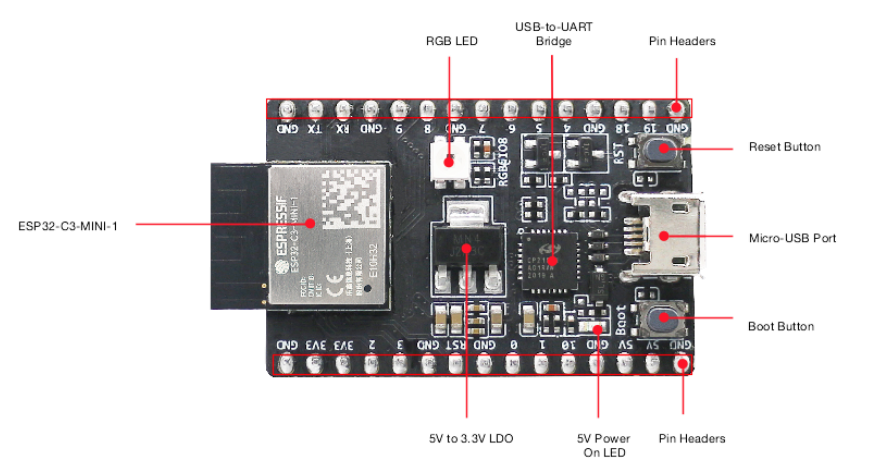
\includegraphics[scale=0.6]{imgs/esp32}
	\caption{Konfiguracija razvojnog sustava ESP32-C3-DevKitM-1 \cite{espressif}}
	\label{fig:esp32}
\end{figure}

Budući da modul ima funkciju RF (engl. \textit{radio frequency}) primopredajnika, podržava protokol Bluetooth s podrškom za velike udaljenosti. Druga važna značajka je podsustav za Wi-Fi, koji omogućava propusnost do 20 Mbps protokolom TCP te maksimalnu propusnost od 30 Mbps koristeći protokol UDP. 

Modul ESP32-C3-MINI-1 bežični je uređaj niske potrošnje energije (engl. \textit{ultra-low-power}) primarno namijenjen razvoju aplikacija koje koriste \textit{Bluetooth Low Energy} (BLE) protokol ili Wi-Fi. Na slici \ref{fig:esp32block} nalazi se blok shema modula sa svim dostupnim značajkama.

\begin{figure}[ht]
	\centering
	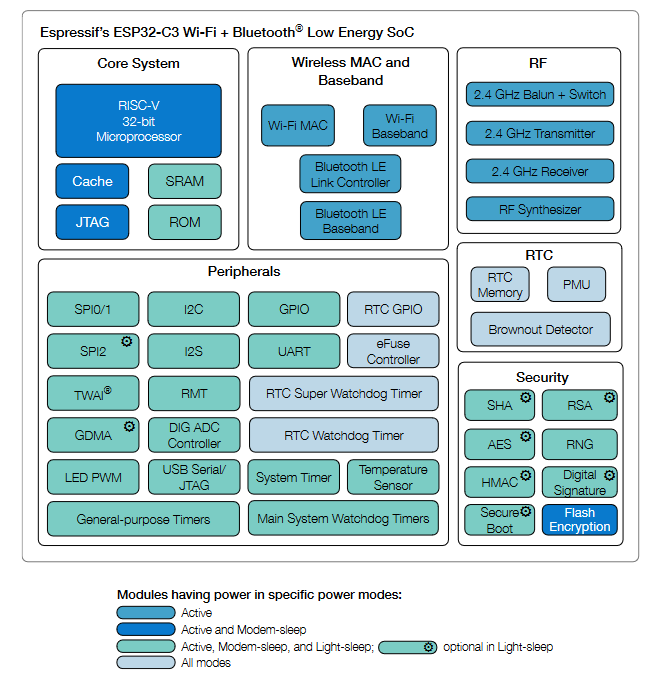
\includegraphics[scale=0.6]{imgs/esp32block}
	\caption{Blok dijagram modula ESP32-C3 \cite{esp32manual}}
	\label{fig:esp32block}
\end{figure}

\section{BLE protokol}

BLE je vrsta bežične komunikacije namijenjena komunikaciji kratkog dometa s niskom potrošnjom energije. Razvijen je kako bi se postigao standard vrlo male snage koji radi s baterijom veličine kovanice (engl. \textit{coin-cell batteries}) nekoliko godina. U odnosu na proizvode koji koriste klasičnu Bluetooth tehnologiju, BLE uređaji troše samo dio energije te omogućavaju malenim uređajima s malim baterijama bežično povezivanje s uređajima koji koriste Bluetooth. BLE protokol ostvaruje nisku potrošnju tako što boravi u stanju mirovanja dok nije povezan s drugim uređajima. Zbog toga može prenositi male količine podataka u kratkom vremenskom periodu. \cite{blevsbluetooth}

BLE radi u istom opsegu od 2,4 GHz kao i standardni Bluetooth, no koristi različite kanale od standardnog Bluetootha. Koristi 40 kanala od 2 MHz za prijenos podataka korištenjem modulacije Gaussova pomaka frekvencije (metoda koja se koristi za glatkije prijelaze između podatkovnih impulsa), zbog čega skokovi frekvencije proizvode manje smetnji u usporedbi sa standardnom Bluetooth komunikacijom.

BLE je tehnologija adaptivnog skakanja frekvencije (engl. \textit{Adaptive frequency hopping} - AFH) koja može koristiti samo podskup svih dostupnih frekvencija kako bi se izbjegle sve frekvencije koje koriste druge neprilagodljive tehnologije. To omogućuje prelazak s lošeg kanala na poznati dobar kanal korištenjem specifičnog algoritma za skakanje frekvencije, koji određuje sljedeći dobar kanal za korištenje. 

Arhitektura BLE tehnologije naziva se još i BLE stog zbog slojevite strukture. Stog se sastoji od dvije glavne komponente: BLE upravljač (engl. \textit{controller}), koji prenosi podatke, te BLE domaćin (engl. \textit{host}), koji definira odnos povezanih uređaja. Prikaz arhitekture stoga nalazi se na slici \ref{fig:ble_stack}.

\begin{figure}[ht]
	\centering
	\includegraphics[scale=0.8]{imgs/ble\_stack}
	\caption{Arhitektura BLE stoga \cite{espressif}}
	\label{fig:ble_stack}
\end{figure}

Osnovni profil koji implementiraju svi Bluetooth uređaji naziva se generički profil pristupa (GAP), koji pruža puni standardni okvir za kontrolu BLE uređaja u komunikacijskim metodama od točke do točke (engl. \textit{point-to-point}) i emitiranju podataka. Profil definira kako BLE uređaji mogu otkriti druge uređaje i povezati se s njima te kako uspostaviti sigurnost i privatnost preko veze. Također detaljno opisuje na koji način uređaji mogu biti odašiljači i promatrači te prenositi podatke bez da su u stanju veze, odnosno bez direktne povezanosti s drugim uređajem. Postoje četiri uloge GAP profila:

\begin{itemize}
	\item emiter (engl. \textit{broadcaster}): šalje oglase,
	\item promatrač (engl. \textit{observer}): prima oglase,
	\item periferija (engl. \textit{peripheral}): uvijek u načinu oglašavanja i u ulozi \textit{slave}, 
	\item centar (engl. \textit{central}): nikada ne šalje oglase, uvijek u \textit ulozi {master}.
\end{itemize}

Generički atributni profil (GATT) odgovoran je za razmjenu podataka i određuje njihovu strukturu. Definira dvije uloge uređaja: GATT poslužitelj i GATT klijent. BLE uređaj može implementirati samo jednu, ili pak istovremeno obje uloge.

GATT poslužitelj najčešće je implementiran u ugradbenom računalu. Poslužitelj implementira tablicu atributa (adresirani dijelovi informacija) strukturiranu u obliku usluga i karakteristika; točnije, sadrži korisne podatke kojima može pristupiti udaljeni klijent. Usluge su skupine karakteristika, odnosno korisničkih podataka koje uređaj želi poslati. Na slici \ref{fig:ble_profile_char} prikazana je opisana hijerarhijska struktura podatkovnog paketa. 

\begin{figure}[ht]
	\centering
	\includegraphics[scale=0.4]{imgs/ble\_profile\_char}
	\caption{Struktura paketa koji se šalju BLE protokolom \cite{ble_profile_char}}
	\label{fig:ble_profile_char}
\end{figure}


BLE protokol nudi tri komunikacijske mogućnosti različitih topologija veze. Prikazane su na slici \ref{fig:ble_com_options}. 

\begin{figure}[ht]
	\centering
	\includegraphics[scale=0.4]{imgs/ble\_com\_options}
	\caption{Komunikacijske mogućnosti u BLE-u \cite{ble_profiles}}
	\label{fig:ble_com_options}
\end{figure}

Prva i najraširenija metoda jest od točke do točke (engl. \textit{point-to-point}). Koristi se u uređajima gdje je povezivanje 1:1, odnosno gdje je moguće međusobno spajanje samo dva uređaja. Većina uređaja u svakodnevnoj uporabi koriste ovu topologiju, primjerice zvučnici, pametne igračke, satovi i uređaji za praćenje zdravlja. Također se naziva i komunikacijom usmjerenom na povezivanje (engl. \textit{connection-oriented communication}), budući da se temelji na povezivanju dvaju uređaja. Iako početna verzija ove metode dopušta spajanje samo dva uređaja, nove verzije protokola omogućuju vezu n:1, što omogućava spajanje više uređaja na jedan centralni uređaj. Razlikuje se od metode emitiranja podataka zbog uloge čvorova u spoju. BLE stog podržava sigurnosnu zaštitu za ovu vrstu topologije 128-bitnim AES algoritmom, no ovom je metodom spajanja zaštita opcionalna. 

U ovom načinu povezivanja uređaji implementiraju jednu od dvije uloge GAP profila, a to su centar i periferija. Centralni je uređaj najčešće onaj koji troši više resursa, primjerice računalo ili mobitel, dok je periferni uređaj ugradbeno računalo s niskom potrošnjom. Nove verzije protokola podržavaju spajanje više perifernih uređaja na centralni.

Iduća metoda je emitiranje podataka (engl. \textit{data broadcast}), čija je topologija povezivanja 1:n. Emitiranje podataka naziva se još i komunikacijom bez povezivanja. Ovo je jednosmjerna metoda komunikacije gdje uređaj emitira svoje podatke svim susjednim uređajima u RF rasponu. Također se koristi za usluge lokacije niske točnosti (margina pogreške od 1,5 metra), primjerice osnovna navigacija u zatvorenom prostoru i pronalaženje puta. Centralni čvor koji emitira podatke još se naziva i BLE odašiljačem. Arhitektura BLE protokola ne podržava sigurnost ovakve vrste povezivanja, no sigurnosni algoritmi se po potrebi mogu implementirati u aplikacijskom sloju. 

Ovaj način povezivanja podržava uloge emitera i promatrača. Pri emitiranju podataka, središnji čvor odnosno odašiljač isporučuje podatke jednosmjernom vezom. Šalje reklamne pakete s podacima u ulozi oglašivača, dok promatrači skeniraju reklamne pakete i tako primaju podatke. Konfiguracija emitiranja podataka najprikladnija je za senzore koji otvoreno emitiraju svoje javne podatke svim zainteresiranim susjednim uređajima. Reklamni se paketi mogu konfigurirati tako da pri njihovu skeniranju promatrač, po potrebi, može zatražiti dodatne informacije od odašiljača posebnim zahtjevom. Paket zahtjeva za skeniranje ne može sadržavati nikakve korisničke podatke.

Postoji nekoliko nedostataka ovakve vrste povezivanja. Ova topologija podržava isključivo jednosmjernu vezu, što znači da odašiljač ne može primiti nikakvu korisnu informaciju od promatrača. Isto tako, svi uređaji u blizini primaju odašiljane pakete, te nije moguće slati podatke samo jednom uređaju. 

Posljednji način jest mrežna topologija (engl. \textit{mesh}). BLE \textit{Mesh} koristi se za uspostavljanje komunikacije više-prema-više uređaja (n:n). Omogućuje stvaranje složenih velikih mreža i idealan je za nadzor, kontrolu i sustave automatizacije gdje je potrebna pouzdana međusobna komunikacija mnoštva uređaja. Ova metoda povećava domet i pokrivenost izvan BLE RF dometa, te pomaže u izbjegavanju fizičkih prepreka. Sigurnost je obavezna u ovom načinu rada, te je podržana BLE stogom. \cite{ble_profiles}

\eject
\chapter{Aplikacijska programska sučelja}

Aplikacijska programska sučelja služe za olakšano korištenje usluga, protokola i periferija koje nudi hardver. Dostupno je mnogo API-ja za ESP32-C3 \cite{espressif}, no ovdje je napravljen osnovni pregled programskih sučelja koja koriste Bluetooth. 

\section{Bluedroid}

\section{NimBLE}

\section{BLE Mesh}

\section{BluFi}

\eject
\chapter{Usporedba API-ja i ograničenja sustava}

\section{Usporedba aplikacijskih sučelja}

Za analizu i usporedbu API-ja odnosno demo aplikacija korištena je mobilna aplikacija \textit{nRF Connect} tvrtke \textit{Nordic Semiconductor}. Pomoću nje moguće je pretražiti i povezati se sa BLE uređajima, kao i komunicirati s njima. Aplikacijom se također mogu analizirati podaci koje uređaj šalje pri oglašavanju te čitati informacije o samim uređajima i uslugama koje nude. \cite{nrfapp}

Jedna od mogućnosti aplikacije je i prikaz RSSI (engl. \textit{Received Signal Strength Indicator}) grafa. To je pokazatelj jačine primljenog signala te služi za mjerenje snage u primljenom radio signalu. RSSI je glavni indikator o jačini signala u danoj točki prostora. RSSI je relativna mjera, stoga je na grafičkom prikazu os RSSI vrijednosti označena dBm skalom, koja je negativna. 

\begin{figure}[ht]
	\begin{minipage}[t]{0.4\textwidth}
		\includegraphics[width=\linewidth]{imgs/graph\_all}
		\label{fig:graph_all}
	\end{minipage}
	\hspace*{\fill}
	\begin{minipage}[t]{0.4\textwidth}
		\includegraphics[width=\linewidth]{imgs/graph\_all2}
		\label{fig:graph_all2}
	\end{minipage}
	\caption{Graf RSSI vrijednosti u ovisnosti o vremenu za \textit{Bluedroid} demo aplikacije}
\end{figure}

\section{Ograničenja razvojnog sustava}

Klasična Bluetooth tehnologija razvijena je kao bežični standard, što je omogućilo razvoj bežičnih i prenosivih uređaja. \textit{BT Classic} tehnologija koristi se za \textit{streaming} aplikacije, poput prijenosa audiozapisa i datoteka. Radi na istim frekvencijama kao i BLE, no ima veći broj RF kanala. Klasični Bluetooth ima veću propusnost podataka, čak do 2.1 Mbps, dok BLE propušta maksimalno 0.27 Mbps. Također ima veću brzinu prijenosa podataka, do 3 Mbps, u usporedbi sa BLE protokolom čija brzina doseže najviše 1 Mbps. Za razliku od BLE protokola čija je glavna odlika niska potrošnja,  zbog brze i nepredvidive komunikacije te složenih postupaka povezivanja \textit{BT Classic} troši znatno više energije i time brže troši bateriju uređaja na kojem se nalazi. Latencija prijenosa je čak 16 puta veća nego u BLE uređajima. Isto tako, podržava samo \textit{peer-to-peer} topologiju, odnosno 1:1, što znači da se istovremeno mogu povezati samo dva uređaja. Detaljnije razlike između verzija Bluetooth protokola nalaze se na slici \ref{fig:blevsbt}. \cite{blevsbt}

\begin{figure}[ht]
	\centering
	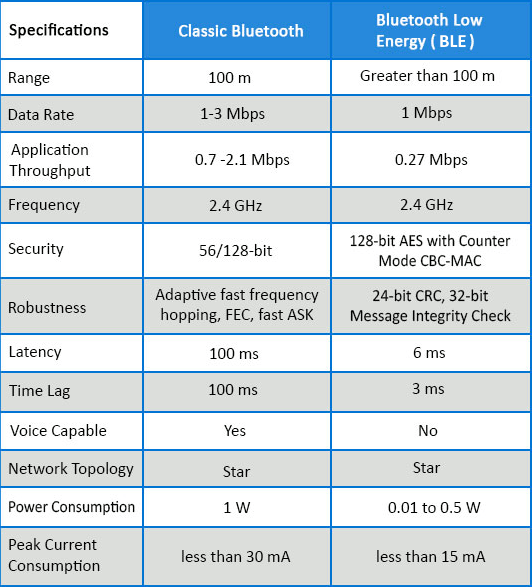
\includegraphics[scale=0.6]{imgs/blevsbt}
	\caption{Razlike između klasične Bluetooth i BLE tehnologije \cite{blevsbt}}
	\label{fig:blevsbt}
\end{figure}

Jedna od mana modula ESP32-C3 jest što ne podržava klasični Bluetooth. Iako BLE nudi prednosti u odnosu na \textit{BT Classic}, poput niske potrošnje i raznovrsnije podržane topologije, uređaji s BLE protokolom i s klasičnom Bluetooth tehnologijom ne mogu međusobno povezati. Ta činjenica ograničava povezivanje i korištenje ESP32-C3 modula, stoga ne može komunicirati s uređajima koji rade na temelju klasičnog Bluetootha. Većina audio uređaja, poput Bluetooth zvučnika, zbog potrebe za prijenosom velike količine podataka koriste klasični Bluetooth radi performansi. ESP32-C3 ne može se povezati s takvim uređajima.



\eject
\chapter{Zaključak}

Zaključak mog seminara.

\eject


\bibliography{literatura}
\bibliographystyle{fer}

\title{Mogućnosti i ograničenja razvojnog sustava ESP32-C3-DevKitM-1 u razvoju Bluetooth aplikacija}
\begin{sazetak}
	TEKST SEMINARA 
	
	\kljucnerijeci{ESP32-C3-DevKitM-1, BLE, Bluetooth API}
\end{sazetak}

\end{document}
